\subparagraph*{Problem explaination}
The goal is the same of the previous problem, but there are few changes in the scenario:
\begin{itemize}
	\item The conversion rates associated to the second item are not known
	\item The number of customers per class is not known
\end{itemize}
\subparagraph*{Strategy}
The script that we have implemented is similar to the previous one: it works on a time horizon of ten days, repeating the experiment ten times. We simulate a random arrival of the customers, providing to them the prices given by the two learners (UCB and TS) for the first item and simulating the purchase of it. In case the customer buys the first item, instead of retrieving the reward of the second item as the product  between the conversion rate of that customer and the respective discounted price, 
we simulate the purchase of it. We calculate the expected reward and we update the learners with the results. 
The algorihm that we have used are the same of the previous one: UCB and TS.

\subparagraph*{Results}
\begin{center}
	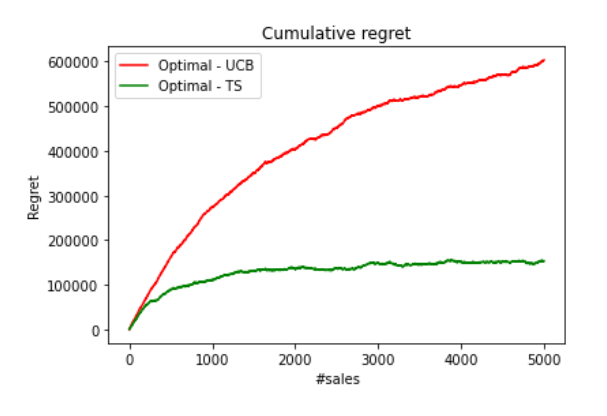
\includegraphics[scale=1]{Images/n4}
\end{center}
\subparagraph*{Considerations}